\documentclass[11pt,letterpaper]{article}
\usepackage[T1]{fontenc}
\usepackage[utf8]{inputenc}
\usepackage{lmodern,microtype}
\usepackage[margin=1.02in,top=.88in,bottom=.88in]{geometry}
\usepackage{amsmath,amssymb,amsthm,mathtools,booktabs,graphicx,xcolor,fancyhdr}
\definecolor{ink}{HTML}{193B52}
\definecolor{accent}{HTML}{875126}
\usepackage[colorlinks=true,linkcolor=ink,citecolor=ink,urlcolor=ink,bookmarksnumbered=true]{hyperref}
\hypersetup{pdftitle={Quadratic characters from finitely many zeros},pdfauthor={Research note prepared for Vladimir Reshetnikov}}
\newtheorem{theorem}{Theorem}[section]
\newtheorem{lemma}[theorem]{Lemma}
\newtheorem{proposition}[theorem]{Proposition}
\newtheorem{corollary}[theorem]{Corollary}
\theoremstyle{remark}\newtheorem{remark}[theorem]{Remark}
\pagestyle{fancy}\fancyhf{}\fancyhead[L]{\small\sffamily\color{ink}Quadratic characters from finitely many zeros}\fancyhead[R]{\small\sffamily\color{ink}Research note}\fancyfoot[C]{\small\thepage}
\setlength{\headheight}{14pt}
\setlength{\parindent}{1.1em}
\setlength{\emergencystretch}{1.4em}
\raggedbottom
\begin{document}
\thispagestyle{plain}
\noindent{\small\sffamily\color{accent} ANALYTIC NUMBER THEORY\quad/\quad NOVEMBER 26, 2026}
\vspace{.40cm}

\noindent{\LARGE\bfseries\color{ink} Quadratic characters from finitely many zeros}\par
\vspace{3pt}
\noindent{\large Sharp bounds for positive dilation averages}\par
\vspace{.35cm}

\noindent\textbf{Abstract.}
For primitive nonprincipal quadratic Dirichlet characters of conductor at most $Q$, we prove that the zeros through a common height $O((\log(2Q))^2\log\log(3Q))$ determine the character. Above twice the constructed cutoff, two distinct characters with the same number of zeros through height $H$ require total ordinate displacement $\gg H/\log(2Q)$ under every matching. The proof reconstructs the individual prime values by rounding a finite sum. The least inert prime also has an exact characterization using only the signs of inner products of interval vectors. A second result determines the shortest positive dilation average that cancels a block of harmonics at several prescribed real parts and multiplicities. We give its unique weights, sharp stability exponent, and exact first-order cost of shortening the averaging interval.

\section{From a critical-line theorem to an inverse question}
Suppose that the conductor of an unknown primitive quadratic character is at most a known number $Q$. How much of its zero spectrum identifies it? A full explicit formula encodes the prime coefficients in the complete infinite spectrum. Our question asks for one finite height that works for every such character, including a margin for error in the ordinates. Throughout, heights are measured by $|\operatorname{Im}\rho|$, logarithms are natural, and zeros are counted with multiplicity.

\paragraph{The sources.}
The readable and compact editions in \cite{repo} rewrite the Alp\"oge--Claude proof. In the pinned readable edition, \texttt{Statements.lean} fixes the statements using Mathlib, and \texttt{Main.lean} gives five theorems. Two state RH in Mathlib's form and its expanded zero-location form. Three give nonvanishing for $\operatorname{Re}s>1/2$ (with the principal pole excepted), critical-line location for open-strip Dirichlet zeros at all positive moduli, and its primitive specialization. In particular every nontrivial-zero term $x^{\rho-1/2}$ is a pure phase $e^{i\gamma\log x}$. Independent checks of the original and shortened developments are documented in \cite{lean,rubin}. For the compact edition, Rubinstein reports a full build, comparison of the five statements against the challenge, and only the standard axioms \texttt{propext}, \texttt{Classical.choice} and \texttt{Quot.sound}. This note uses the formal conclusion as an input. Its new arguments are given below as mathematical proofs.

The proof guide and \texttt{OneSidedBound.lean} identify a more specific point of contact. Short integral forms, a spanning argument, and a lower bound on heights of integral forms enter a comparison of covolumes. Cancellation of the common main term produces an upper bound on a smoothed prime remainder. Its weight contains $\Lambda(n)(1-\chi_d(n))(1/n-1/x)$ on a selected residue class, emphasizing inert primes. An analytic pole criterion turns this family of bounds into Dirichlet nonvanishing \cite{repo}. The Wikipedia exposition describes the classical explicit formula in the other direction, expressing prime-power counts through zeros \cite{wiki}. We use that direction to locate the first inert prime and then to distinguish characters quantitatively. The auxiliary theta lifts are used upstream in the formal proof of GRH.

\paragraph{How the two results are related.}
Both arguments use averaging on a logarithmic scale. A positive weight can isolate one prime power in the explicit formula. On the other side of that formula, dilating the argument multiplies a complex power by a phase and a real amplitude. This raises a separate extremal question about the width required to cancel selected oscillations without using negative weights. Sections~\ref{sec:spectral} and~\ref{sec:decode} give the inverse arithmetic results. Sections~\ref{sec:filters} and~\ref{sec:harmonics} solve the extremal problem.


\section{The least inert prime from signs of interval pairings}\label{sec:spectral}

Let $\chi$ be a primitive nonprincipal quadratic Dirichlet character of
conductor $q$ and parity $\kappa=(1-\chi(-1))/2$. Write
$p_-(\chi)=\min\{p\text{ prime}:\chi(p)=-1\}$. Factoring any positive integer on which $\chi$ takes the value $-1$ proves that such a prime exists.
For a Legendre character it is the least positive quadratic nonresidue among units.
For the character of a quadratic field it is the least inert prime.

Use Dirichlet GRH to write the nontrivial zeros of $L(s,\chi)$ as
$1/2+i\gamma$, listing both signs with multiplicity. For a compact interval
$I$ of positive length define a vector with one coordinate per zero,
\[
 v_I(\gamma)=\int_I e^{i\gamma x}\,dx,\qquad
 C_\chi(I,J)=\operatorname{Re}\sum_{\gamma}
                  \overline{v_I(\gamma)}v_J(\gamma).
\]
A zero with $\gamma=0$ contributes $|I|\,|J|$ to the pairing.
The vectors belong to $\ell^2$ because
$|v_I(\gamma)|\leq\min(|I|,2/|\gamma|)$ for $\gamma\ne0$ and the
zero count is $O_q(T\log(2+T))$ \cite{zeroct}. Thus the signs below are
signs of real Hilbert-space inner products, and the series converges
absolutely. Put $J-I=\{y-x:x\in I,\ y\in J\}$.

\begin{theorem}[Sign threshold]\label{thm:signthreshold}
Let $R_\chi$ be the supremum of all $R>0$ for which
$C_\chi(I,J)<0$ for every pair of compact intervals of positive length
satisfying $J-I\subset (0,R)$. Then
\[
                        R_\chi=\log p_-(\chi).
\]
For every $R>R_\chi$ there are equal-length intervals with
$J-I\subset(0,R)$ and $C_\chi(I,J)>0$, of arbitrarily short length.
\end{theorem}

\subsection*{The explicit formula away from the origin}

Set $g_{I,J}(u)=|I\cap(J-u)|$, where vertical bars denote length. This
nonnegative trapezoid, which is a triangle for equal interval lengths, is
supported on $J-I$ and has integral $|I|\,|J|$. Define
\[
       K_\kappa(u)=\frac{\exp[-(\kappa+1/2)u]}{1-\exp(-2u)}
       \qquad (u>0).
\]
For $J-I\subset(0,\infty)$ the explicit formula gives
\begin{equation}\label{eq:packetweil}
 C_\chi(I,J)=-\int_0^\infty g_{I,J}(u)K_\kappa(u)\,du
        -\sum_{n\ge2}\frac{\Lambda(n)\chi(n)}{\sqrt n}\,
                         g_{I,J}(\log n).
\end{equation}
Here $\Lambda(p^k)=\log p$ and $\Lambda(n)=0$ away from prime powers.
The sum on the right is finite.

For a derivation, first let $g$ be smooth with compact support in
$(0,\infty)$ and use $H(t)=\int_0^\infty g(u)\cos(tu)\,du$ in
the Guinand--Weil formula for a primitive character \cite[eq.~(2.1)]{weilref}.
With $\widehat H(\xi)=\int_{\mathbb R}H(t)e^{-2\pi i t\xi}\,dt$,
Fourier inversion gives $\widehat H(0)=0$ and
$\widehat H(\pm u/(2\pi))=\pi g(u)$ for $u>0$.
This removes the conductor term and gives the prime sum in
\eqref{eq:packetweil}. The gamma term is
\[
 \frac{1}{2\pi}\int_{\mathbb R}H(t)\operatorname{Re}\psi
       \left(\frac14+\frac\kappa2+\frac{it}{2}\right)dt,
 \qquad \psi=\Gamma'/\Gamma.
\]
In the standard integral for $\psi(z)$, the term depending on $t$ is
$-e^{-zv}/(1-e^{-v})\,dv$. Terms independent of $t$ integrate to zero.
Truncating the $v$-integral first, using Fourier inversion, and putting
$v=2u$ gives $-\int gK_\kappa$. The truncations stabilize after the
Fourier inversion because $g$ has compact support away from zero.
For $g=g_{I,J}$, its cosine transform at $t$ is
$\operatorname{Re}(\overline{v_I(t)}v_J(t))$. Convolve $g$ with a smooth
even nonnegative approximate identity of support small enough to keep the
convolution in $(0,\infty)$. Its cosine transform is the original one
times a multiplier bounded in absolute value by one. Uniform convergence
on the common compact support and the summable bound on the zero side
then give \eqref{eq:packetweil}.

\begin{proof}[Proof of Theorem~\ref{thm:signthreshold}]
For $J-I\subset(0,\log p_-(\chi))$, every prime power $p^k$
in the sum has $p<p_-(\chi)$ and hence $\chi(p^k)\ge0$. Since
$K_\kappa>0$ and $g_{I,J}$ has positive integral, the pairing is strictly
negative.

For the opposite direction put $r=\log p_-(\chi)$,
$I_h=[0,h]$, $J_{r,h}=[r,r+h]$. The weight is
$g_{I_h,J_{r,h}}(u)=(h-|u-r|)_+$.
For sufficiently small $h>0$, its support lies in $(0,R)$ and contains
just one logarithm of a prime power. The prime contributes
$h\log p_-(\chi)/\sqrt{p_-(\chi)}$. The absolute value of the gamma
term is at most $h^2K_\kappa(r-h)$ because $K_\kappa$ is decreasing.
The pairing is positive for all sufficiently small $h$.
\end{proof}

\subsection*{Isolating one prime and bounding the omitted zeros}

Write $C_\chi(r,h)=C_\chi(I_h,J_{r,h})$. For $r=\log n$, where
$n=p^k$, choose $0<h<\log(1+1/n)$. This explicit condition isolates
$\log n$ from the logarithms of all other integers and ensures $r-h>0$.
Put
\[
 A_\kappa(r,h)=\int_{r-h}^{r+h}(h-|u-r|)K_\kappa(u)\,du.
\]
Equation~\eqref{eq:packetweil} gives the exact identity
\begin{equation}\label{eq:packetrecover}
 \chi(n)=-\frac{\sqrt n}{h\log p}
       \bigl(C_\chi(\log n,h)+A_\kappa(\log n,h)\bigr).
\end{equation}
Thus the correction at either parity is explicit. At a ramified prime the
corrected quantity is exactly zero.

For a height cutoff $T$, the portion of $C_\chi(r,h)$ with $|\gamma|\le T$
is particularly simple:
\[
 C_{\chi,T}(r,h)=\sum_{|\gamma|\le T}
       \frac{4\sin^2(\gamma h/2)}{\gamma^2}\cos(\gamma r),
\]
with the summand at zero defined by continuity as $h^2$. Uniformly in $r,h$
and $T\ge2$,
\begin{equation}\label{eq:packettail}
   |C_\chi(r,h)-C_{\chi,T}(r,h)|
           \le \frac{16(\log(qT)+1)}{T}=:E_q(T).
\end{equation}
Indeed Corollary~1.2 of \cite{zeroct} gives
$N(t)\le(t/\pi)\log(qt/(2\pi e))+0.298\log(qt)+4.358$,
where $N(t)$ counts nontrivial zeros with $|\gamma|\le t$. In particular
$N(t)\le 2t\log(qt)$ for $q\ge3$ and $t\ge2$.
The tail is bounded by $4\sum_{|\gamma|>T}|\gamma|^{-2}
\le8\int_T^\infty N(t)t^{-3}\,dt$, proving \eqref{eq:packettail}.
If $E_q(T)<h\log p/(2\sqrt n)$, replacing $C_\chi$ by $C_{\chi,T}$
in \eqref{eq:packetrecover} and rounding to the nearest integer recovers
$\chi(n)$ exactly. A computation using enclosures for the zeros and the
gamma integral must include their numerical errors in the same margin.

A smaller bound, useful at moderate heights, follows by retaining the
lower endpoint in the partial summation. Write $b(t)=0.298\log(qt)+4.358$.
Then
\begin{equation}\label{eq:betterpacket}
 |C_\chi(r,h)-C_{\chi,T}(r,h)|\le
 \frac{4(\log(qT/(2\pi))+1)}{\pi T}
 +\frac{4(2b(T)+0.149)}{T^2}.
\end{equation}
To see this, substitute $N(t)=(t/\pi)\log(qt/(2\pi e))+D(t)$,
$|D(t)|\le b(t)$, in
$4[-N(T)/T^2+2\int_T^\infty N(t)t^{-3}dt]$.
The main term integrates exactly. The bound for $D$ gives the second term,
since $2\int_T^\infty t^{-3}\log(t/T)\,dt=1/(2T^2)$.

\paragraph{An odd character at height 100.}
Take the character modulo $3$, $r=\log 2$, and $h=3/8$.
Equation~\eqref{eq:betterpacket} gives a tail bound below $0.06687$,
smaller than $h\log 2/(2\sqrt2)>0.09189$. The supplied script found
46 positive ordinates up to $100$ and obtained the same count by
numerically tracking the argument of $L(s,\chi)$.
It gives $C_{\chi,100}=0.10863420$ and
$A_1(r,h)=0.07200989$, and the full arithmetic side is $0.11178851$.
The resulting estimate of $\chi(2)$ is $-0.98283822$, which rounds to
$-1$. The cutoff bound and the rounding criterion are proved inequalities.
The decimal evaluations and the list of ordinates use ordinary
multiprecision arithmetic.

The spectral Hilbert-space viewpoint also occurs in Suzuki's work on the screw function of the Riemann zeta function \cite{suzuki}. Here the observable is the sign for two separated intervals.

\begin{figure}[htbp]\centering
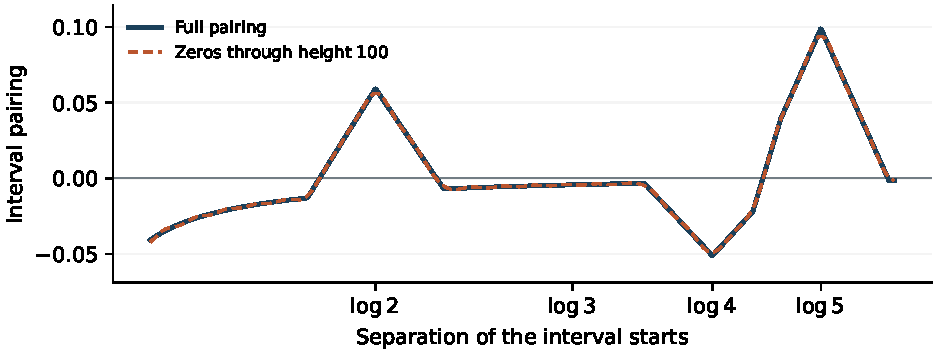
\includegraphics[width=.89\linewidth]{interval_pairing.pdf}
\caption{The quadratic character modulo $3$, with equal interval lengths $0.14$. The positive peaks are centered at $\log 2$ and $\log 5$. At $\log 4$ the prime-square coefficient has the opposite sign, and the ramified prime $3$ produces no peak. The threshold in Theorem~\ref{thm:signthreshold} concerns the whole interval of differences, whose right endpoint is the plotted separation plus $0.14$.}
\end{figure}


\section{Determining a quadratic character from finitely many zeros}\label{sec:decode}

A triangular test already recovers one value of $\chi$ by rounding.
A higher convolution power suppresses the tail much faster. The resulting
test uses the same list of zeros for every prime power up to a prescribed
bound. Even the parity correction can be absorbed into the rounding margin.

Let $Q\ge q$, $X\ge2$, $h=1/(8X)$. Choose an even integer $r\ge2$, put
$T=2r/h=16rX$, and increase $r$ until
\begin{equation}\label{eq:choose}
  2^r\ \ge\ \frac{32}{\log 2}\,r\sqrt X\log(eQT).
\end{equation}
Write $f$ for the probability density obtained by convolving $r$ copies of the uniform density on $[-h/r,h/r]$. Thus $f$ is supported on $[-h,h]$ and its transform in angular frequency is
$\widehat f(t)=\operatorname{sinc}(ht/r)^r$, where $\operatorname{sinc} y=\sin(y)/y$ and $\operatorname{sinc}(0)=1$.

\begin{theorem}[Finite recovery with a rounding margin]\label{thm:decode}
Let $\Gamma$ be the multiset of ordinates of all the nontrivial zeros of $L(s,\chi)$ with $|\gamma|\le T$, for a primitive nonprincipal quadratic character of conductor at most $Q$. For each $n=p^a\le X$, $a\ge1$, form
\begin{equation}\label{eq:finite}
  B(n;\Gamma)=-\frac{\sqrt n}{(\log p)f(0)}
       \sum_{\gamma\in\Gamma}\cos(\gamma\log n)
                      \operatorname{sinc}(h\gamma/r)^r.
\end{equation}
Rounding $B(n;\Gamma)$ to the nearest integer gives $\chi(n)$, including the value zero at ramified primes. The conclusion holds simultaneously for all such $n$. It still holds with approximate ordinates $\widetilde\gamma$, one for each occurrence of $\gamma$, whenever
\begin{equation}\label{eq:perturb}
 \sum_{\gamma\in\Gamma}|\widetilde\gamma-\gamma|
 \ \le\ \frac{\log 2}{16\sqrt X\,h(\log X+h)} .
\end{equation}
One can take $T\ll X\bigl(\log(2X)+\log\log(3Q)\bigr)$ with an absolute implied constant.
\end{theorem}

\begin{proof}
The convolution of the first $r/2$ uniforms is an even density $v$ of total mass one on an interval of length $h$. Consequently $f(0)=\int v^2\ge1/h$ by Cauchy--Schwarz. For $n\le X$, the gap from $\log n$ to the next larger integer logarithm is at least $\log(1+1/n)\ge1/(n+1)>h$, and the gap on the other side is larger. In the explicit formula of Section~\ref{sec:spectral} take $g(u)=f(u-\log n)$. The same mollification argument applies since $\widehat f(t)=O_{h,r}((1+|t|)^{-r})$. Exactly one prime power contributes. The infinite version of the sum inside \eqref{eq:finite} is
\[
   -\frac{\chi(n)\log p}{\sqrt n}\,f(0)
          -\int f(u-\log n)K_\kappa(u)\,du.
\]
Throughout this integral, $K_\kappa(u)\le n^{-1/2}e^{h/2}/(1-e^{2h}/n^2)<2/\sqrt n$, since $n\ge2$, $h\le1/16$. The normalized contribution of this integral has absolute value at most $2h/\log2$.

Next write $N(t)=\#\{\gamma:|\gamma|\le t\}$ with multiplicity. From $N(t)\le2t\log(Qt)$ for $t\ge2$ and Stieltjes integration by parts,
\begin{align*}
 \sum_{|\gamma|>T}|\widehat f(\gamma)|
 &\le \left(\frac rh\right)^r r\int_T^\infty
                        \frac{N(t)}{t^{r+1}}\,dt\\
 &\le \frac{2r}{r-1}\,T\left(\frac{r}{hT}\right)^r
             \left(\log(QT)+\frac{1}{r-1}\right)
 \le 4 T\log(eQT)2^{-r}.
\end{align*}
Multiplying by $\sqrt n/((\log p)f(0))$ and invoking \eqref{eq:choose} bounds the normalized tail by $1/4$. In particular
\[
  |B(n;\Gamma)-\chi(n)|\le\tfrac14+2h/\log 2.
\]
Finally $\cos(t\log n)\widehat f(t)=\int f(u-\log n)\cos(tu)\,du$ has Lipschitz constant at most $\log X+h$. The perturbations in \eqref{eq:perturb} cost at most another $1/16$ after normalization. Since $1/4+1/(8\log2)+1/16<1/2$, rounding is unambiguous in all cases.

For the height bound let $L=\log(2X)+\log\log(3Q)$. The logarithm of the right side of \eqref{eq:choose} is at most $C(L+\log(2r))$ for an absolute $C$, using $T=16rX$. An even $r$ between $AL$ and $AL+2$ satisfies \eqref{eq:choose} for a sufficiently large absolute $A$.
\end{proof}

\begin{corollary}[Separation of the zero multisets]\label{cor:identity}
For $Q\ge3$ there is a common cutoff
\[
    T_Q\ \ll\ (\log(2Q))^2\log\log(3Q)
\]
such that the nontrivial zero ordinates in $[-T_Q,T_Q]$, including their multiplicities, uniquely determine every primitive nonprincipal quadratic character of conductor at most $Q$. All constants are absolute.
\end{corollary}

\begin{proof}
Put $M=\operatorname{lcm}(q_1,q_2)\le Q^2$ for any two conductors under consideration. Distinct primitive quadratic characters induce distinct characters on $(\mathbb Z/M\mathbb Z)^\times$, by uniqueness of the primitive inducing character. Their product there has a proper kernel. Under Dirichlet GRH the least prime outside that kernel is $O((\log(2M))^2)$, coprime to $M$, by the subgroup theorem of Lamzouri, Li and Soundararajan \cite[Thm.~1.1]{lls}, enlarging the absolute constant for small moduli. At this prime the two character values differ.
Choose a common $X=C(\log(2Q))^2$ with $C$ sufficiently large, and choose $r,T_Q$ as in Theorem~\ref{thm:decode}. The finite sum recovers the distinguishing prime value and therefore distinguishes the two spectra.
\end{proof}

\begin{theorem}[Separation at every higher cutoff]\label{thm:displacement}
Let $X,r,h,T$ be as in Theorem~\ref{thm:decode}, and $H\ge2T$.
Suppose two primitive nonprincipal quadratic characters of conductor at
most $Q$ have different values at some prime $p\le X$. If their zero
multisets in $[-H,H]$ have the same cardinality, then every
bijection between the lists, counting individual occurrences, satisfies
\[
        \sum_{\gamma}|\gamma-\gamma'|>
                         \frac{H}{144\pi\sqrt X}.
\]
In particular, for distinct such characters one can take
$X=C(\log(2Q))^2$ as in Corollary~\ref{cor:identity}, giving
$\sum |\gamma-\gamma'|\gg H/\log(2Q)$ at every $H\ge2T$ for
which the cardinalities agree.
\end{theorem}

\begin{proof}
Refine the compactly supported density $f$ of Theorem~\ref{thm:decode}
by setting $B=H/8$ and
$\phi(u)=f(u)\operatorname{sinc}^2(Bu)/f(0)$.
Since $f=v*v$ with $v$ even, Cauchy--Schwarz gives $f(u)\le f(0)$.
Thus $\phi(0)=1$ and $\int\phi\le\min(h,\pi/B)$, using both
$f(0)\ge1/h$ and $\int_{\mathbb R}\operatorname{sinc}^2(Bu)\,du=\pi/B$.
The transform of $\phi$ is the average of $\widehat f(t+V)/f(0)$
where $V$ is the sum of two independent uniforms on $[-B,B]$.
If $|t|>H$, then $|t+V|\ge3|t|/4$.

Use $\phi(u-\log p)$ in the same explicit formula. The gamma term
after multiplication by $\sqrt p/\log p$ is at most $2h/\log 2$.
The zero-tail estimate in Theorem~\ref{thm:decode}, with
$|\widehat\phi(t)|\le (4r/(3h|t|))^r/f(0)$, bounds the normalized
tail by
\[
 \frac{4h\sqrt X}{\log 2}\,H\log(eQH)
                  \left(\frac{4r}{3hH}\right)^r.
\]
This decreases for $H\ge2T$. At $H=2T$ the ratio to the earlier tail bound is
\[2(2/3)^r\frac{\log(2eQT)}{\log(eQT)}<1,\]
since \eqref{eq:choose} implies $r\ge4$. Thus the tail is at most
$1/4$. Finally the normalized spectral test
$(\sqrt p/\log p)\int\phi(u-\log p)\cos(tu)\,du$ has Lipschitz
constant at most
$\sqrt X(1+h/\log 2)\pi/B\le9\pi\sqrt X/H$.
A matching of total displacement at most $H/(144\pi\sqrt X)$ adds at
most $1/16$ to the decoding error. The bound
$1/4+2h/\log2+1/16<1/2$ forces the two
prime values to agree by rounding, a contradiction.
\end{proof}

Banks compares zeros of distinct primitive Dirichlet characters in intervals starting at large height \cite{banks}. Banks and Loftus study unshared zeros in high windows \cite{loftus}. Here the observations start at the real axis, the conductors can differ, and the estimate controls the total displacement in a matching. The proof gives a sufficient cutoff. Determining the optimal height remains a separate question.

\paragraph{Four coefficients from one list.}
For $q=Q=3$ and $X=5$ the rule gives $r=14$, $h=1/40$ and $T=1120$. Our calculation found 941 positive ordinates, in agreement with a separately sampled horizontal argument count. Using each ordinate and its negative in \eqref{eq:finite} gives the following values.
\begin{center}
\begin{tabular}{lrrrr}\toprule
Prime power $n$ & $2$ & $3$ & $4$ & $5$ \\
\midrule
Finite sum $B(n;\Gamma)$ & $-0.990596$ & $0.003337$ & $1.003759$ & $-0.998733$\\
Nearest integer & $-1$ & $0$ & $1$ & $-1$\\
\bottomrule\end{tabular}
\end{center}
The zero sum alone returns the character at the ramified prime and the expected sign change between $2$ and $2^2$. The script evaluates the $L$-function by Euler--Maclaurin summation and checks sample values with independent Hurwitz-zeta evaluation. Root enumeration and decimal arithmetic in this example are numerical. The proof of Theorem~\ref{thm:decode} uses the complete mathematical multiset.


\section{How short can a positive dilation average be?}\label{sec:filters}

A dilation of a power $x^s$ by $e^u$ multiplies it by $e^{su}$. Thus a probability measure $\mu$ on the logarithmic scale acts on that power by the multiplier
\[
 F_\mu(s)=\int e^{su}\,d\mu(u).
\]
Positivity preserves inequalities between the quantities being averaged. It also places an exact restriction on the zeros of the multiplier. We determine the restriction, the unique measure attaining equality, and the first-order cost of making its interval shorter.

Fix $\tau>0$, distinct real numbers $\beta_1,\ldots,\beta_r$, and positive integers $m_1,\ldots,m_r$. Put $s_j=\beta_j+i\tau$, $m=\sum_jm_j$, $h=\pi/\tau$, and $b=mh$. Throughout this section $\mu$ is a compactly supported Borel probability measure on $\mathbb R$. We require
\begin{equation}\label{eq:fjets}
 F_\mu^{(k)}(s_j)=\int u^k e^{s_ju}\,d\mu(u)=0
 \qquad (1\le j\le r,\ 0\le k<m_j).
\end{equation}
These are conditions on the multiplier. Even when a zero of an $L$-function is multiple, its logarithmic derivative has a simple pole. Higher multiplier orders can instead enforce insensitivity to small errors in the location of a zero.

\begin{theorem}[Minimum width and all equality cases]\label{thm:fwidth}
Any measure satisfying \eqref{eq:fjets} has support diameter at least $m\pi/\tau$. Up to translation, exactly one measure has that diameter. It is $\mu_* = \sum_{\ell=0}^m w_\ell\delta_{\ell h}$, with
\begin{equation}\label{eq:fpoly}
 \sum_{\ell=0}^m w_\ell z^\ell
 =\prod_{j=1}^r \left(\frac{z+e^{h\beta_j}}{1+e^{h\beta_j}}\right)^{m_j}.
\end{equation}
\end{theorem}

\begin{proof}
Use the real vector space
\[
 V=\operatorname{span}_{\mathbb R}\{u^k e^{\beta_j u}:1\le j\le r,\ 0\le k<m_j\}.
\]
It has dimension $m$. Indeed, division by the largest exponential and passage to $+\infty$ in a putative linear relation forces its polynomial coefficient to be zero, and induction removes the remaining terms. A nonzero $p\in V$ has at most $m-1$ real zeros counting multiplicities. For the induction on $m$, divide $p$ by $e^{\beta_1 u}$ and differentiate. The result lies in a space of the same form with dimension $m-1$ because the first polynomial loses one degree. If the derivative vanishes identically the quotient is constant. Otherwise Rolle's theorem, including multiplicities, gives the bound from the induction hypothesis.

There is consequently a nonzero $q\in V$ with zeros at $h,2h,\ldots,(m-1)h$. These $m-1$ linear conditions have a solution, all its prescribed zeros are simple, and it has no further real zeros. Its solution space is one-dimensional, since otherwise two independent solutions could be combined to vanish also at $0$. For $m=1$ the list of prescribed zeros is empty. Choose its sign to make
\begin{equation}\label{eq:fexposer}
 g(u)=q(u)\sin(\tau u)\ge0\quad(0\le u\le b).
\end{equation}
Its zeros consist precisely of the grid $G=\{0,h,\ldots,b\}$. The endpoints are simple and the interior zeros are double.

Translation multiplies $F_\mu(s)$ by a nowhere vanishing exponential, preserving zero orders. If a solution has diameter at most $b$, translate its left endpoint to $0$. By the imaginary parts of \eqref{eq:fjets}, $\int g\,d\mu=0$. Positivity forces $\mu$ onto $G$. Write $P(z)=\sum w_\ell z^\ell$ for its weight polynomial. Since $F_\mu(s)=P(e^{hs})$ and the inner map has nonzero derivative, $P$ must vanish at each $-e^{h\beta_j}$ to order at least $m_j$. These distinct roots account for $m$ degrees. Normalization $P(1)=1$ now gives \eqref{eq:fpoly}. Conversely, all the coefficients in that product are positive, they sum to one, and its transform satisfies \eqref{eq:fjets}. Both endpoint masses are positive, giving the claimed width.
\end{proof}

For quantitative statements, fix $I=[0,b]$. Use the $2m$ real coordinates
\[
 Y(u)=\big(\operatorname{Re}(u^k e^{s_ju}),\operatorname{Im}(u^k e^{s_ju})\big)_{j,k}.
\]
Choose any norm $\|\cdot\|$ on this coordinate space, with dual norm $\|\cdot\|_*$. Define $\varepsilon(\mu)=\|\int Y\,d\mu\|$. For example, the maximum of the moduli of the $m$ complex coordinates measures the largest jet error. The first Wasserstein distance $W_1$ is the minimum expected displacement over all couplings of two probability measures.

\begin{proposition}[Sharp stability on the critical interval]\label{prop:fwasser}
For all probability measures supported on $I$ with $\varepsilon(\mu)\le 1$,
\[
 W_1(\mu,\mu_*)\le C\,\varepsilon(\mu)^\alpha,
 \qquad
 \alpha=\begin{cases}1,&m=1,\\[1mm]1/2,&m\ge2.\end{cases}
\]
The constant depends only on the prescribed jets and the norm. In each case the exponent is best possible.
\end{proposition}

\begin{proof}
Write $g=v\cdot Y$ as in \eqref{eq:fexposer}. Its zero orders and compactness give $g(u)\ge c\,\operatorname{dist}(u,G)^2$ on $I$. If $m=1$ they give $g(u)\ge c\,\operatorname{dist}(u,G)$. Since $\int g\,d\mu\le\|v\|_*\varepsilon(\mu)$, nearest-node rounding sends $\mu$ to a measure $\nu$ on $G$ at mean cost $O(\varepsilon^\alpha)$, using Cauchy--Schwarz in the quadratic case. Each feature is Lipschitz on $I$, so $\varepsilon(\nu)=O(\varepsilon^\alpha)$.

The map from real signed weights on $G$ to their total mass and the real parts of their $m$ jets is invertible. At the nodes the imaginary parts vanish, and the kernel would give a polynomial of degree at most $m$ divisible by the numerator in \eqref{eq:fpoly}, with value zero at $1$. Such a polynomial is zero. The fixed inverse gives $\sum_\ell |\nu(\{\ell h\})-w_\ell|=O(\varepsilon^\alpha)$. Moving the excess masses by at most $b$ and using the triangle inequality proves the result.

For $m\ge2$, split any interior atom of $\mu_*$ into equal masses at distances $\eta$ to either side, with $0<\eta<h/2$. Taylor's theorem gives $\varepsilon=O(\eta^2)$. Rounding attains transport cost $w_\ell\eta$, and every transport to $G$ costs at least the expected distance to $G$. For $m=1$, moving the left atom to $\eta$ gives distance $w_0\eta$ and jet error $O(\eta)$. These families rule out every larger exponent.
\end{proof}

\begin{theorem}[First-order cost of shortening the interval]\label{thm:fleak}
For $0<d<b$, let
\[
 I_d=[d/2,b-d/2],\qquad D(d)=\min_{\operatorname{supp}\mu\subset I_d}\varepsilon(\mu).
\]
If $g=v\cdot Y$ is the certificate in \eqref{eq:fexposer}, then
\begin{equation}\label{eq:fleak}
 \lim_{d\downarrow0}\frac{D(d)}d
   =\frac{w_0g'(0)-w_mg'(b)}{2\|v\|_*}>0 .
\end{equation}
\end{theorem}

\begin{proof}
Normalize $v$ to dual norm $1$, scaling $g$ accordingly. The convex hull of $Y(I_d)$ is compact and consists exactly of the possible moment vectors. Separation of a convex set from the open norm ball about the origin gives
\begin{equation}\label{eq:fdual}
 D(d)=\max_{\|z\|_*\le1}\ \min_{u\in I_d} z\cdot Y(u).
\end{equation}
Indeed each inner minimum is bounded by the distance to the convex set. A supporting hyperplane separating the set from the open ball of that radius gives the reverse inequality when the distance is positive, and $z=0$ handles zero distance.

We first determine the supporting directions at $d=0$. Suppose $z\cdot Y\ge0$ on $I$. Since its integral under $\mu_*$ vanishes, $z\cdot Y$ vanishes at every node. Write
\[
 z\cdot Y(u)=p(u)\cos(\tau u)+r(u)\sin(\tau u),\qquad p,r\in V.
\]
Node values force $p$ to vanish at $m+1$ points, so $p=0$. At each interior node the derivative must also vanish, giving $r(\ell h)=0$. Thus $r$ is a multiple of $q$, and positivity selects a nonnegative multiple. Independence of the basis of $V$ then gives $z=\lambda v$, $\lambda\ge0$.

Set $a_0=g'(0)/2$, $a_m=-g'(b)/2$ and $a_\ell=0$ for $0<\ell<m$. Write $K=\sum_\ell w_\ell a_\ell$. The endpoint zeros are simple, so $K>0$. Choose a maximizer $z_d$ in \eqref{eq:fdual}. Along any convergent subsequence as $d\downarrow0$ its limit is nonnegative on $Y(I)$, since $D(d)\ge0$ and interior points eventually belong to $I_d$. Thus the limit equals $\lambda v$, $0\le\lambda\le1$. Evaluate $z_d\cdot Y$ at the grid points with only the two endpoints moved inward by $d/2$. Its minimum is at most the average with weights $w_\ell$. The original weighted sum is zero. Taylor expansion at the two ends, with remainder uniform for bounded $z_d$, gives $\limsup D(d)/d\le K$ by subsequence compactness.

For the lower bound, the map $p\mapsto((-1)^\ell p(\ell h))_{\ell=0}^m$ from $V$ into $\mathbb R^{m+1}$ has rank $m$ by the zero count. Its image is the hyperplane orthogonal to $(w_0,\ldots,w_m)$ by the real moment equations for $\mu_*$. Consequently we may prescribe
\[
 (-1)^\ell p(\ell h)=K-a_\ell
 \qquad(0\le\ell\le m).
\]
Consider $g_d(u)=g(u)+d\,p(u)\cos(\tau u)$. On fixed small endpoint neighborhoods it remains monotone toward the interior as measured from each endpoint, and at the two new endpoints it has value $dK+O(d^2)$. Near an interior node $x_\ell=\ell h$, its value is at least
\[
 c|u-x_\ell|^2+dK-Cd|u-x_\ell|\ \ge\ dK-O(d^2).
\]
Off these neighborhoods $g$ has a strictly positive minimum. The coefficient vector of $g_d$ has dual norm $1+O(d)$. Its normalization in \eqref{eq:fdual} gives $D(d)\ge dK-O(d^2)$, proving \eqref{eq:fleak}.
\end{proof}

\paragraph{A computable constant.}
Take $\tau=\pi$, $(\beta_1,\beta_2)=(0,\log 2)$, and $m_1=m_2=1$. The extremal weights are $(1/3,1/2,1/6)$. Choose $g(u)=(2-2^u)\sin(\pi u)$. For the maximum of the two complex moduli, the dual norm of its coefficient vector is $2+1=3$. As $g'(0)=\pi$ and $g'(2)=-2\pi$, \eqref{eq:fleak} gives $D(d)=(\pi/9)d+o(d)$.

\paragraph{Relation to earlier results.}
Logan's real even extremal case yields a power of a cosine \cite{logan}. Half-period spacing and binomial filters for repeated zeros at a single oscillator frequency are classical in vibration input shaping \cite{kang,singhose}. The width lower bound alone also follows from Obrechkoff's polynomial sector bound \cite{obre}. For a measure on $[0,L]$, $L>0$, round its support to the mesh $L/N$. The resulting transforms $P_N(e^{sL/N})$ converge locally uniformly to $F_\mu$, with $P_N$ of degree at most $N$ and nonnegative coefficients. For each small $\eta>0$, disjoint disks about the two conjugate sets of target zeros contain at least $2m$ zeros counting multiplicities for large $N$, by Rouch\'e's theorem. Their exponential images count as distinct roots with multiplicity, since the exponential is injective on the bounded region of interest for large $N$. They lie in the sector of half-angle $(\tau+\eta)L/N$, which permits at most $2(\tau+\eta)L/\pi$ roots. Letting $\eta$ decrease to zero gives the width bound. Positive-measure reconstruction by dual certificates and Wasserstein estimates has a general theory \cite{eft}. Here the common ordinate allows the support, extremal weights for arbitrary real parts and multiplicities, sharp stability exponent, and shortening constant to be determined together. The minimum in \eqref{eq:fleak} uses a fixed origin and a centered shortening. Translating the interval can change the numerical size of nonzero derivatives.


\section{A block of consecutive harmonics}\label{sec:harmonics}

The same average can cancel a whole band of harmonics at each prescribed real part. For a single undamped frequency band with simple conditions, the extremal interval length is dual to the sharp zero-gap theorem of Kozma and Oravecz \cite{kozma}. Here each real part may have a different prescribed multiplicity. A residue formula gives a certificate for the whole band and determines the sensitivity at the extremal interval.

\begin{theorem}[Consecutive harmonics with independent real parts and multiplicities]\label{thm:hblock}
Fix integers $p,H\ge1$, a frequency $\tau>0$, distinct real numbers $\beta_j$, and positive integers $m_j$. Write
\[
 B=2p+H-1,\qquad h=\frac{2\pi}{B\tau},\qquad n=H\sum_jm_j,
 \qquad a_j=e^{h\beta_j},\qquad \omega=e^{2\pi i/B}.
\]
Suppose a compactly supported probability measure $\mu$ satisfies
\begin{equation}\label{eq:hjets}
 F_\mu^{(k)}(\beta_j+i\ell\tau)=0
 \quad(p\le\ell\le p+H-1,\;0\le k<m_j,\;\text{all }j).
\end{equation}
The least possible support diameter is $b=nh$. The unique minimizer up to translation has masses $w_t$ at $th$, $0\le t\le n$, where
\begin{equation}\label{eq:hpoly}
 \sum_{t=0}^n w_t z^t = \frac{P(z)}{P(1)},\qquad
 P(z)=\prod_j\left[\prod_{\ell=p}^{p+H-1}(z-a_j\omega^\ell)\right]^{m_j}.
\end{equation}
When $p=1$ the inner polynomial is $\sum_{t=0}^H a_j^{H-t}z^t$. In particular, for $p=H=1$ this recovers Theorem~\ref{thm:fwidth}.
\end{theorem}

\begin{proof}
First, each factor of degree $H$ in \eqref{eq:hpoly} has strictly positive coefficients. Put $\theta_s=(2s-H+1)\pi/B$ for $0\le s<H$. Its roots are $-a_je^{i\theta_s}$. Let $R(y)=\prod_s(1+ye^{i\theta_s})=\sum c_ty^t$, so that the factor is $a_j^H R(z/a_j)$ by symmetry and $\sum_s\theta_s=0$. With $\alpha=e^{i\theta_0}$, the identity $(1+\alpha y)R(\omega y)=(1+\alpha\omega^H y)R(y)$ gives $c_0=1$ and
\[
 \frac{c_t}{c_{t-1}}=\frac{\sin((H-t+1)\pi/B)}{\sin(t\pi/B)}>0 \qquad (1\le t\le H).
\]
Here $H<B$. The transform of the proposed measure is $P(e^{hs})/P(1)$. Its roots give \eqref{eq:hjets} with the required multiplicities.

For the converse, translate to $[0,b]$ and use the dimensionless coordinate $u=x/h$. Form a second polynomial of degree $n$,
\[
 Q(z)=\prod_j\prod_{s=0}^{H-1}(z-a_je^{i\theta_s})^{m_j}.
\]
Its roots occur in conjugate pairs or on the positive real axis. With the principal logarithm define
\[
 E(u)=\sum_{v:\,Q(v)=0}^{\rm distinct}\operatorname*{Res}_{z=v}\frac{z^{u-1}}{Q(z)},
 \qquad g(x)=(-1)^{n+1}\sin(\pi u)E(u).
\]
At a pole $v=a_je^{i\theta_s}$ of order $m_j$ its residue is $v^u$ times a polynomial in $u$ of degree at most $m_j-1$. Conjugation shows $E$ is real for real $u$. Multiplication by $\sin(\pi u)$ replaces the arguments $\theta_s$ by $\theta_s\pm\pi$. After dividing by $h$ the resulting frequencies are $(p+s)\tau$ and $-(p+H-1-s)\tau$. Consequently $g$ is a real linear combination of the real and imaginary parts of the tests in \eqref{eq:hjets}.

For $0<u<n$, integrate $z^{u-1}/Q(z)$ along a keyhole contour enclosing the poles, slit along the negative axis. The outer and inner circle integrals are respectively $O(R^{u-n})$ and $O(\delta^u)$. On the two banks of the slit the powers differ by $-2i\sin(\pi u)t^{u-1}$ at $z=-t$. Since $Q(-t)=(-1)^n|Q(-t)|$ for $t>0$, the residue theorem gives
\begin{equation}\label{eq:hcert}
 E(u)=\frac{(-1)^{n+1}\sin(\pi u)}{\pi}
 \int_0^\infty\frac{t^{u-1}}{|Q(-t)|}\,dt .
\end{equation}
The integral is finite and strictly positive. Thus $g$ is positive between grid nodes and has a double zero at each interior node. Directly at the endpoints, $E(0)=-1/Q(0)$ by accounting for the pole at zero, and $E(n)=1$ by the residue at infinity. The endpoint zeros of $g$ are simple.

Now \eqref{eq:hjets} implies $\int g\,d\mu=0$, hence $\mu$ is supported on the grid. Its mass polynomial must have the $n$ roots, counted with multiplicity, prescribed by $P$. Indeed the distinct $a_j$ give disjoint circles, the $H$ roots on each circle are distinct, and $e^{hs}$ has nonvanishing derivative. A polynomial of degree at most $n$ with those zeros is a scalar multiple of $P$. Normalization fixes the scalar. Positivity of both endpoint masses then excludes every smaller diameter.
\end{proof}

\paragraph{Stability and shortening.}
Let $Y$ collect the $2n$ real and imaginary test functions in \eqref{eq:hjets}. On $[0,b]$ use any fixed norm for the moment error $\varepsilon=\|\int Y\,d\mu\|$ as in Section~\ref{sec:filters}, and write $g=v\cdot Y$. Then Proposition~\ref{prop:fwasser} holds with the optimal exponent $1/2$ for $n\ge2$ and $1$ for $n=1$. The centered shortening formula is likewise
\[
 \lim_{d\downarrow0}\frac{1}{d}\min_{\operatorname{supp}\mu\subset[d/2,b-d/2]}\varepsilon(\mu)
 =\frac{w_0g'(0)-w_ng'(b)}{2\|v\|_*}>0.
\]
For the certificate above, $g'(0)=\pi/(h|Q(0)|)$ and $g'(b)=-\pi/h$. The monic polynomial in \eqref{eq:hpoly} satisfies $w_0/w_n=|Q(0)|=\prod_j a_j^{Hm_j}$. Thus each endpoint contributes equally, and the displayed slope simplifies to $\pi w_n/(h\|v\|_*)$.

Here are the linear-algebra details needed to apply those proofs. Exponential polynomials with distinct complex exponents and the stated polynomial multiplicities are linearly independent because the differential operators $(D-\lambda)^k$ successively eliminate the other components and act invertibly on a surviving component with a different exponent. Thus the test space has real dimension $2n$. Evaluation on the $n+1$ grid nodes has rank $n$, since the annihilating signed grid vectors correspond by the root argument to the one-dimensional space of multiples of $P$. Its image is exactly the hyperplane perpendicular to $(w_t)$, so every prescribed perturbation of node values in that hyperplane can be interpolated.

The kernel of grid evaluation consists exactly of $\sin(\pi u)q(u)$, where $q$ ranges over the real exponential-polynomial space generated by $u^k(a_je^{i\theta_s})^u$, $k<m_j$, taking conjugate coefficients for conjugate nodes. The same frequency calculation gives containment, and both spaces have dimension $n$. If a test is nonnegative, its zero integral under the extremizer forces all its grid values to vanish. Its derivative vanishes at the interior nodes, hence $q(1)=\cdots=q(n-1)=0$. These conditions leave exactly one dimension because evaluation of $q$ at $1,\ldots,n$ is invertible. For instance the sequences $u^kv^u$ obey the order-$n$ recurrence with polynomial $Q$ and nonzero constant term. Vanishing at $n$ consecutive integers gives zero at all integers. The sequences are independent, as their generating functions for nonnegative integer arguments have distinct poles $1/v$ with pole orders $1,\ldots,m_j$. This also covers $n=1$. The nonnegative supporting tests consequently form the ray generated by $g$. The zero orders in \eqref{eq:hcert} now give the transport bound by nearest-grid rounding as in Proposition~\ref{prop:fwasser}. Interpolating the endpoint losses and using the unique supporting ray gives the claimed coefficient by Theorem~\ref{thm:fleak}.

\paragraph{Two examples.}
For $p=1$, $H=2$, $h=1$, $\beta=0$, and a single simple condition at each harmonic, the two frequencies are $2\pi/3$ and $4\pi/3$. The unique shortest filter places mass $1/3$ at each of $0,1,2$. For the same two frequencies choose instead $e^{\beta_1}=1/2$, $e^{\beta_2}=2$ with multiplicities $1,2$. The optimal width is $6$, and its polynomial and masses are
\[
 \frac{(4z^2+2z+1)(z^2+2z+4)^2}{343},
 \qquad (w_0,\ldots,w_6)=\frac{(16,48,108,92,57,18,4)}{343}.
\]
The roots on the inner circle are simple and those on the outer circle are double. The accompanying exact-arithmetic check verifies all six moment equations.



\paragraph{Application to a prime sum.}
Let $W$ be smooth with compact support in $(1,2)$ and let $S_W(x)=\sum_n\Lambda(n)W(n/x)$ for $x>1$. In the smoothed explicit formula a nontrivial zeta zero $\rho$ contributes $-x^\rho\widetilde W(\rho)$, where $\widetilde W(s)=\int_0^\infty W(y)y^{s-1}\,dy$ \cite[Thm.~7.1]{green}. A positive finite average of $S_W(xe^u)$ therefore multiplies this contribution by $F_\mu(\rho)$ and the leading term by $F_\mu(1)$. For any zero $\rho=1/2+i\gamma$ with $\gamma>0$, put $h=\pi/\gamma$. The combination
\[
 \frac{e^{h/2}S_W(x)+S_W(e^hx)}{1+e^{h/2}}
\]
cancels the conjugate pair exactly. Taking its $m$-fold dilation average gives an order-$m$ zero in the multiplier and uses a logarithmic span $mh$, minimal by Theorem~\ref{thm:fwidth}. If a frequency is displaced by $\eta$, this multiplier at the displaced zero is $O(|\eta|^m)$ as $\eta\to0$. No assumption on simplicity is needed. This example uses the actual zero ordinate. The block theorem also applies to prescribed harmonic frequencies whether or not they occur as ordinates of zeta zeros.


\paragraph{Scope of the novelty claim.}
The classical inputs include the explicit formula, zero counting, the least-prime-outside-a-subgroup theorem, and the single-layer extremal results cited above. The finite rounding rule, its uniform displacement consequence, and the simultaneous weighted harmonic-block theorem with its shortening law are the formulations developed here. The cited literature provides comparisons. Publication priority for these precise statements has not been established.

\section*{Further research questions}
\begin{enumerate}
\item Can the factor $\log\log(3Q)$ be removed from the cutoff for identifying a primitive quadratic character? The individual-prime tests pay for isolation at the spacing of adjacent integer logarithms. A test that uses several distinguishing primes at once could give a different scale.
\item For primitive characters of bounded order greater than two, what separation of low zeros suffices to distinguish the complex character values, including the conjugate pair? The real cosine pairing used here loses phase information.
\item For which sets of nonconsecutive prescribed frequencies does the shortest positive average still have an explicitly computable support and shortening constant? The common grid and the one-dimensional family of nonnegative supporting functions are special properties used in the consecutive case.
\end{enumerate}

\begin{thebibliography}{99}\small
\bibitem{repo} L. Sernau and collaborators, \emph{GRH for Dirichlet $L$-functions, in Lean 4}, commit \texttt{72fead102f663d5c7a407964a13dc0cf9d977207}. \href{https://github.com/lsernau/grh-lean/tree/72fead102f663d5c7a407964a13dc0cf9d977207}{Repository}, \href{https://github.com/lsernau/grh-lean/blob/72fead102f663d5c7a407964a13dc0cf9d977207/grh/src/Statements.lean}{statements}, \href{https://github.com/lsernau/grh-lean/blob/72fead102f663d5c7a407964a13dc0cf9d977207/grh/src/Main.lean}{theorems}, \href{https://github.com/lsernau/grh-lean/blob/72fead102f663d5c7a407964a13dc0cf9d977207/grh/GUIDE.md}{reading guide}, \href{https://github.com/lsernau/grh-lean/blob/72fead102f663d5c7a407964a13dc0cf9d977207/grh/src/New/Reduction/OneSidedBound.lean}{one-sided bound}.
\bibitem{lean} Lean FRO and Mathlib Initiative, \href{https://leanprover-community.github.io/blog/posts/riemann-hypothesis/}{\emph{Lean verification of the Riemann Hypothesis}}, November 2026.
\bibitem{rubin} M. Rubinstein, \href{https://www.math.uwaterloo.ca/~mrubinst/alpoge_claude_grh/}{\emph{Alp\"oge/Claude proof of the Generalized Riemann Hypothesis}}, verification results for the original and compact editions, November 21 and 26, 2026.
\bibitem{wiki} Wikipedia contributors, \href{https://en.wikipedia.org/wiki/Riemann_hypothesis}{\emph{Riemann hypothesis}}, consulted November 26, 2026. See the formulation, explicit formula and Dirichlet generalization.
\bibitem{weilref} A. Chirre, V. J. Pereira J\'unior and D. de Laat, \href{https://doi.org/10.1090/mcom/3638}{\emph{Primes in arithmetic progressions and semidefinite programming}}, Math. Comp. (2021), equation (2.1).
\bibitem{zeroct} M. A. Bennett, G. Martin, K. O'Bryant and A. Rechnitzer, \href{https://doi.org/10.1090/mcom/3599}{\emph{Counting zeros of Dirichlet $L$-functions}}, Math. Comp. 90 (2021), 1455--1482, Corollary 1.2.
\bibitem{lls} Y. Lamzouri, X. Li and K. Soundararajan, \href{https://arxiv.org/abs/1309.3595}{\emph{Conditional bounds for the least quadratic non-residue and related problems}}, Math. Comp. 84 (2015), 2391--2412, Theorem 1.1.
\bibitem{banks} W. D. Banks, \href{https://arxiv.org/abs/2302.07073}{\emph{Comparing zeros of distinct Dirichlet $L$-functions}}, Theorem 1.1.
\bibitem{loftus} W. D. Banks and K. Loftus, \href{https://arxiv.org/abs/2607.22930}{\emph{Unshared zeros of Dirichlet $L$-functions}}, preprint (2026).
\bibitem{green} B. Green, \href{https://people.maths.ox.ac.uk/greenbj/papers/primenumbers.pdf}{\emph{The Prime Number Theorem}}, Oxford lecture notes, Chapter 7.
\bibitem{suzuki} M. Suzuki, \href{https://doi.org/10.1112/jlms.12785}{\emph{Aspects of the screw function corresponding to the Riemann zeta-function}}, J. Lond. Math. Soc. (2023).
\bibitem{obre} A. Eremenko and A. Fryntov, \href{https://arxiv.org/abs/1409.4849}{\emph{Remarks on the Obrechkoff inequality}}, Proc. Amer. Math. Soc. 144 (2016), 703--707.
\bibitem{kang} B. B. Kang, \href{https://doi.org/10.1371/journal.pone.0276669}{\emph{Specified-duration shapers for suppressing residual vibrations}}, PLOS ONE 17 (2022), e0276669.
\bibitem{singhose} M. A. Lau and L. Y. Pao, \href{https://doi.org/10.1016/S0005-1098(03)00024-4}{\emph{Input shaping and time-optimal control of flexible structures}}, Automatica 39 (2003), 893--900.
\bibitem{eft} A. Eftekhari, J. Tanner, A. Thompson, B. Toader and H. Tyagi, \href{https://arxiv.org/abs/1804.01490}{\emph{Sparse non-negative super-resolution---simplified and stabilised}}, Appl. Comput. Harmon. Anal. 50 (2021), 216--280.
\bibitem{logan} B. F. Logan, \href{https://doi.org/10.1137/0514024}{\emph{Extremal problems for positive-definite bandlimited functions. III. The maximum number of zeros in an interval $[0,T]$}}, SIAM J. Math. Anal. 14 (1983).
\bibitem{kozma} G. Kozma and F. Oravecz, \href{https://arxiv.org/abs/math/0601021}{\emph{On the gaps between zeros of trigonometric polynomials}}, Real Anal. Exchange 28 (2002/03), 447--454.
\end{thebibliography}
\end{document}
